%%%%%%%%%%%%%%%%%%%%%%%%%%%%%%%%%%%%%%%%%%%%%%%%%%%%%%%%%%%%%%%%%%%%%
%
% talk intro optimization Cotonou 2022
%
%%%%%%%%%%%%%%%%%%%%%%%%%%%%%%%%%%%%%%%%%%%%%%%%%%%%%%%%%%%%%%%%%%%%%

\documentclass[12pt]{beamer}
\usepackage[utf8]{inputenc}
\usepackage{amsmath}
\usepackage{amsfonts}
\usepackage{amssymb}
\usepackage{graphicx}
\graphicspath{{figures/}{Figures/}}
%\usepackage{beamerthemesplit}
%\usepackage{beamerthemeshadow} 
\usepackage{color}
\usepackage{hyperref}
\usepackage{xspace}
\usepackage{xifthen}
\usepackage{multicol}
\usepackage{mathtools}
\usepackage{algorithm,algorithmicx}
\usepackage{algcompatible}
\usepackage{bbm}
\usepackage{textcomp}
\usepackage{yfonts}

\usepackage{tikz}
\usetikzlibrary{calc,shapes,arrows}

% custom commands in sty file, for easier writting and change of notations
\usepackage{my_notations}
\newcommand*{\mmds}{\enm{\text{MMD}^2}}

\usetheme{Madrid}
\usecolortheme{beaver}

%%%%%%%%%%%%%%%%%%%%%%%%%%%%%%%%%%%%%%%%%%%%%%%%%%%%%%%%%%%%%%%%%%%%%
\begin{document}
\title
[Optimization: multi-tasker or utopia?
%\hspace{0.1cm} \insertframenumber/\inserttotalframenumber
]
{Optimization for quantitative decisions: a versatile multi-tasker or an utopia?}
\author
[R. Le Riche]
{\large Rodolphe Le Riche$^{*}$}
\institute[CNRS LIMOS]{$^*$~CNRS at LIMOS (Mines Saint Etienne, UCA) France
} 
\date[July 2022]{25 July 2022 \\
Cotonou, Benin, IA summer school 
\\\vskip\baselineskip
{\small Acknowledgements : Vallet foundation, Bernard Guy}
} 
\begin{frame}
\titlepage
\end{frame}

%=======================================================================================
%\begin{frame}[allowframebreaks]
%\frametitle{Content} 
%\begin{multicols}{2}
%\tableofcontents[currentsection]
%\end{multicols}
%\end{frame}


%=======================================================================================
\begin{frame}[allowframebreaks]
\frametitle{The advent of optimization algorithms}
\begin{minipage}[b]{0.25\textwidth}
\centering
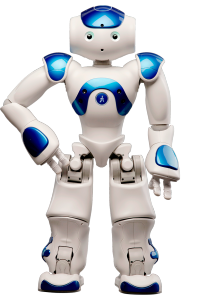
\includegraphics[width=0.4\textwidth]{Figures/NAO.png}
\\ ``Intelligence'' =
\end{minipage} 
\hfill
\begin{minipage}[b]{0.2\textwidth}
{\scriptsize \cite{bachoptimization}}
\vskip 2cm
~
\end{minipage} 
\\
\hfill
\begin{minipage}[t]{0.2\textwidth}
\centering
 models + 
\\
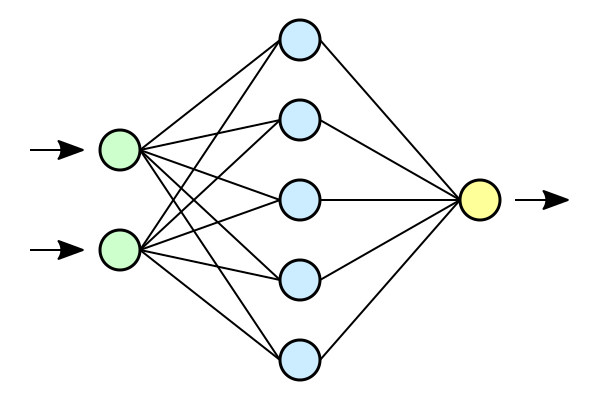
\includegraphics[width=\textwidth]{Figures/neural_network.png} 
\end{minipage} 
\begin{minipage}[t]{0.2\textwidth}
\centering
\textbf{\textcolor{red}{algorithms}} + 
\\
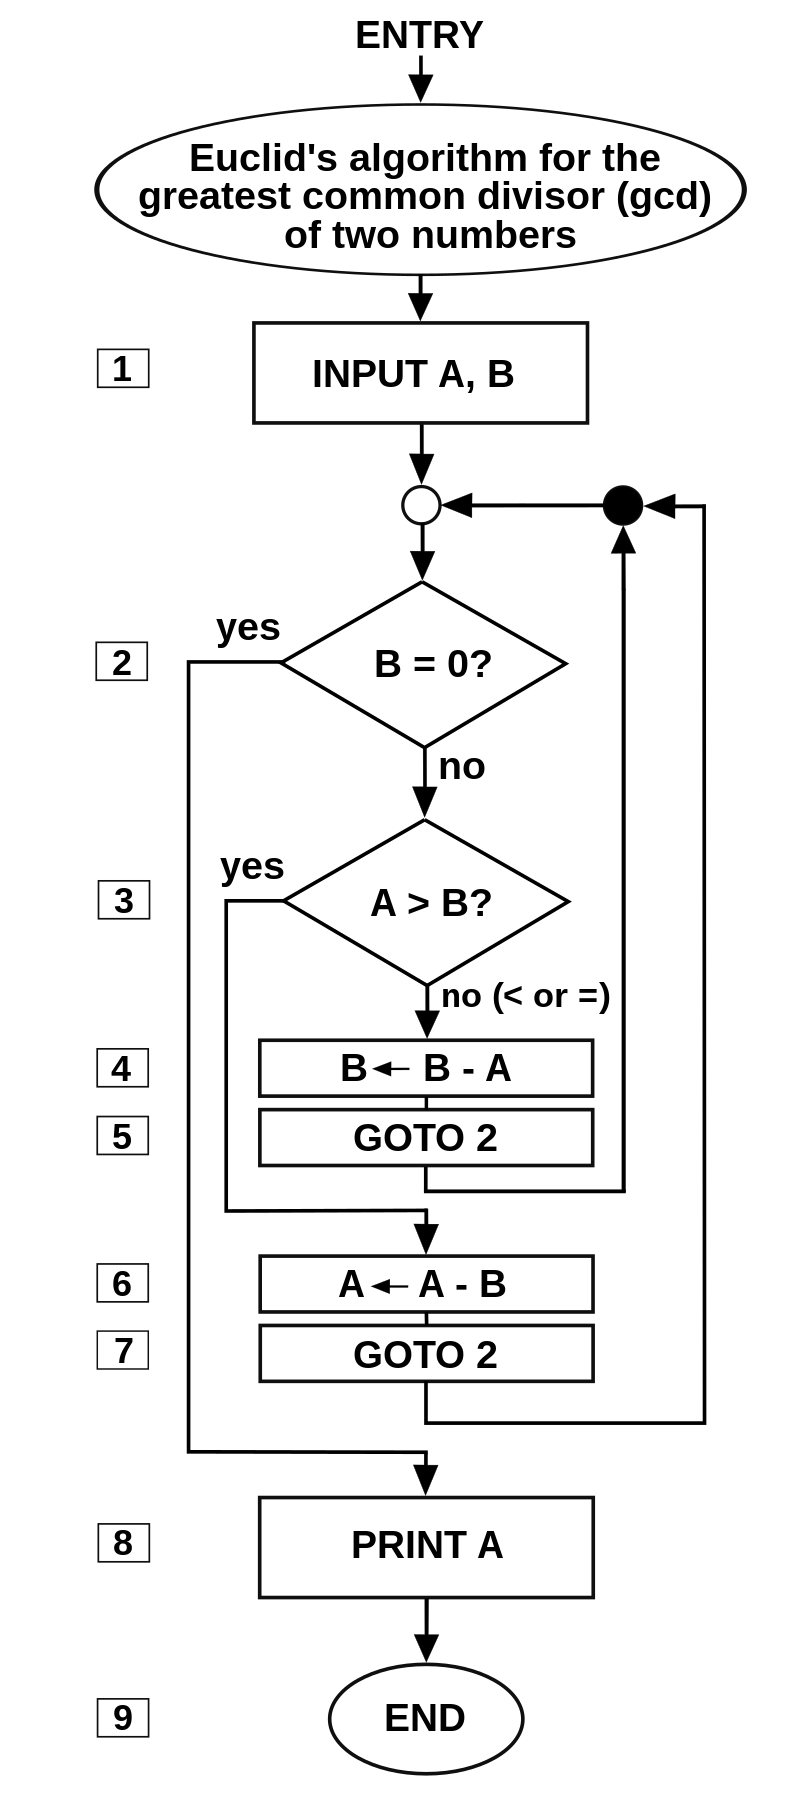
\includegraphics[width=0.5\textwidth]{Figures/algorithm.png} 
\end{minipage} 
\begin{minipage}[t]{0.2\textwidth}
\centering
data + 
\\\vskip 0.2cm

\includegraphics[width=\textwidth]{Figures/data.png} 
\end{minipage} 
\begin{minipage}[t]{0.2\textwidth}
\centering
computing power 
\\\vskip 0.2cm
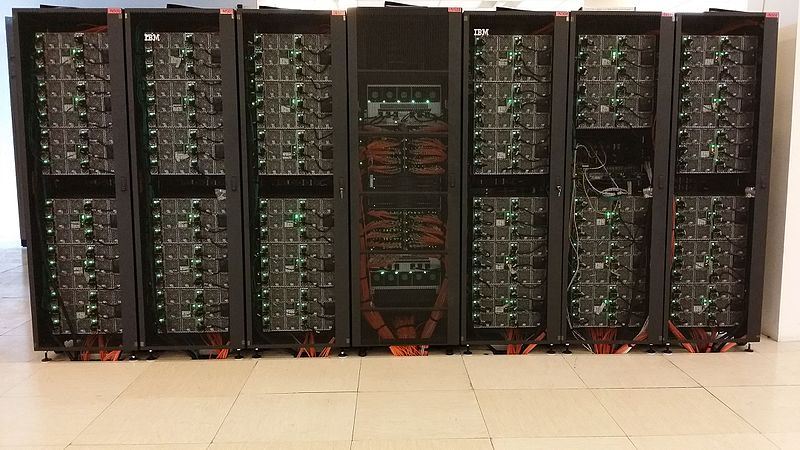
\includegraphics[width=\textwidth]{Figures/supercomputer.jpg} 
\end{minipage} 
\newpage
There are numerous conferences$^\star$ (and journals) where new optimization algorithms are presented, whether in 
\begin{itemize}
\item applied mathematics. Ex: {\scriptsize SIAM Conf. on Optimization, FGS (French-German-Swiss) workshops series, PGMO Days, \ldots}
\item computer science (including machine learning). Ex: {\scriptsize LION (Learning and Intelligent OptimizatioN conf.), EURO (EURopean Operational research soc.) conf., Optimization days, NEURIPS, \ldots}
\item or in application fields. Ex: {\scriptsize SIAM Conf. on Uncertainty Quantification (statistics), AIAA/MAO (Multidisciplinary Analysis and Optimization) or WCSMO (World Congress on Structural and Multidisciplinary Optimization) conferences (engineering), ECCOMAS (aeronautics), ICASP (civil engineering), \ldots}
\end{itemize}
\hfill($^\star$ {\scriptsize : arbitrarily listing some of the meetings I participated to} )
\newpage
Some recent algorithms are highly cited, i.e., are seen as key technological components : 
\begin{itemize}
\item NAG (\cite{nesterov1983method}, 1983, $>5500$ citations),
\item CMA-ES (\cite{hansen2001completely}, 2001, $>4100$ citations),
\item ADAGRAD (\cite{duchi2011adaptive}, 2011, $>10400$ citations),
\item RMSprop (\cite{tieleman2012lecture}, 2012, $>6000$ citations),
\item Adam (\cite{kingma2014adam}, 2014, $>113000$ citations),
\item \ldots
\end{itemize}
\end{frame}


%=======================================================================================
\begin{frame}
\frametitle{}
\centering
{\usebeamerfont*{frametitle}\usebeamercolor[fg]{frametitle} 
Optimization algorithms? 
\vskip\baselineskip
What are we talking about?
}
\end{frame}

%%%%%%%%%%%%%%%%%%%%%%%%%%%%%%%%%%%%%%%%%%%%%%%%%%%%%%%%%%%%%%%%%%
\begin{frame}[allowframebreaks]
\frametitle{The fundamental optimization problem}
\begin{minipage}{\textwidth}
\begin{minipage}{0.5\textwidth}
\centering
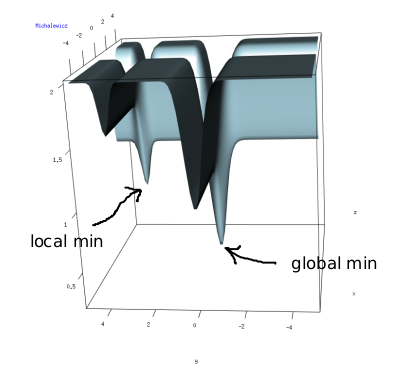
\includegraphics[width=0.9\textwidth]{michalewicz_local_global.png} \\
\vspace{-0.4cm}
{\small (2D continuous example)}
\end{minipage}
\begin{minipage}{0.45\textwidth}
Find the lowest point of a function,
\begin{equation*}
\min_{x \in \mathcal S } f(x)
\end{equation*}
\end{minipage}
\vskip\baselineskip
Looks easy on this drawing. \\
But the function is known pointwise, each evaluation costs computer time, and $\mathcal S$ may be complex (high-dimensional, non-continuous, constrained \ldots)
\end{minipage}
\newpage
\begin{minipage}{0.45\textwidth}
\centering
\begin{tikzpicture}
\node[anchor=south west,inner sep=0, outer sep=0] (contour) at (0,0) {
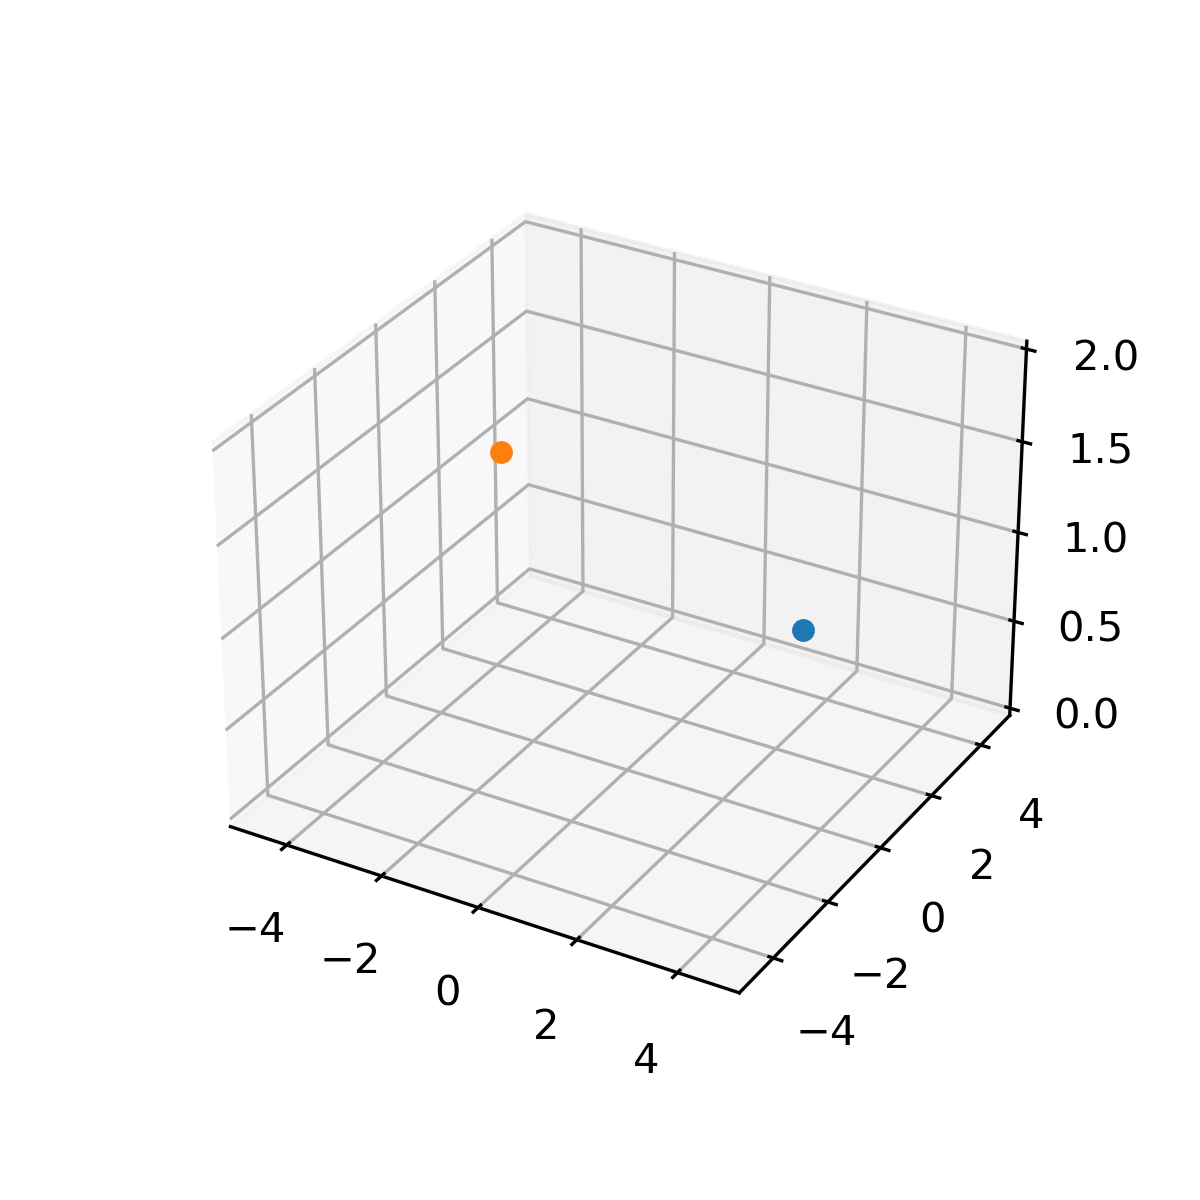
\includegraphics[width=0.9\textwidth]{two_3D_points.png}
};
\begin{scope}[x={(contour.south east)},y={(contour.north west)}]
%\draw[help lines,xstep=0.1,ystep=0.1] (0,0) grid (1,1);
\node[] (xstar) at (0.73,0.5) {$\widehat{x^\star}$};
\node[] (xprime) at (0.37,0.65) {$x'$};
\end{scope}
\end{tikzpicture}
\vspace{-0.4cm}
{\small (what the random optimizer sees)}
\end{minipage}
\hfill
\begin{minipage}{0.45\textwidth}
Random search \hfill ~\\
\noindent\rule{\textwidth}{1pt}
{\scriptsize
\begin{algorithmic}%[1]
\REQUIRE $x^\text{LB},~x^\text{UB},t^\text{max}$
\STATEx $t \leftarrow 0,~\widehat{f^\star} \leftarrow + \infty$
\WHILE{$t<t^\text{max}$}
\STATE $x' \leftarrow \mathcal U[x^\text{LB},~x^\text{UB}]\quad$ \COMMENT{uniform law}
\STATE calculate $f(x')$, $t \leftarrow t+1$
\IF{$f(x')<\widehat{f^\star}$}
\STATE $\widehat{x^\star}\leftarrow x' \quad,\quad \widehat{f^\star} \leftarrow f(x')$
\ENDIF
\ENDWHILE
\STATE \textbf{return} $\widehat{x^\star}, \widehat{f^\star}$
\end{algorithmic}
}
\vspace{-0.8\baselineskip}
\noindent\rule{\textwidth}{1pt}
\end{minipage}
\end{frame}


%%%%%%%%%%%%%%%%%%%%%%%%%%%%%%%%%%%%%%%%%%%%%%%%%%%%%%%%%%%%%%%%%
\begin{frame}[allowframebreaks]
\frametitle{Optimization = a quantitative formulation of decision}
Optimization is a way of mathematically modeling decision.
\vskip\baselineskip
\mbox{
\begin{minipage}[c]{0.3\textwidth}

\includegraphics[width=\textwidth]{decision-clipart.jpg}
\end{minipage}
\begin{minipage}[c]{0.7\textwidth}
\begin{equation*}
\min_{x \in \mathcal S} f(x)
\end{equation*}
\begin{itemize}
\item $x$ vector of decision parameters (variables)~: dimensions, investment, tuning of a machine / program, \ldots
\item $f(x)$~: decision cost, minus $\times$ performance, \ldots 
\item $\mathcal S$~: set of possible values for $x$, search space
\end{itemize}
\end{minipage}
} % end mbox
\newpage
\vskip 2cm
{\large
\begin{center}
A versatile approach to problem solving.
\vskip\baselineskip
Examples :
\end{center}
}
\end{frame}

%%%%%%%%%%%%%%%%%%%%%%%%%%%%%%%%%%%%%%%%%%%%%%%%%%%%%%%%%%%%%%%%%
\begin{frame}
\frametitle{Optimization example: aircraft global pre-design}
\begin{center}
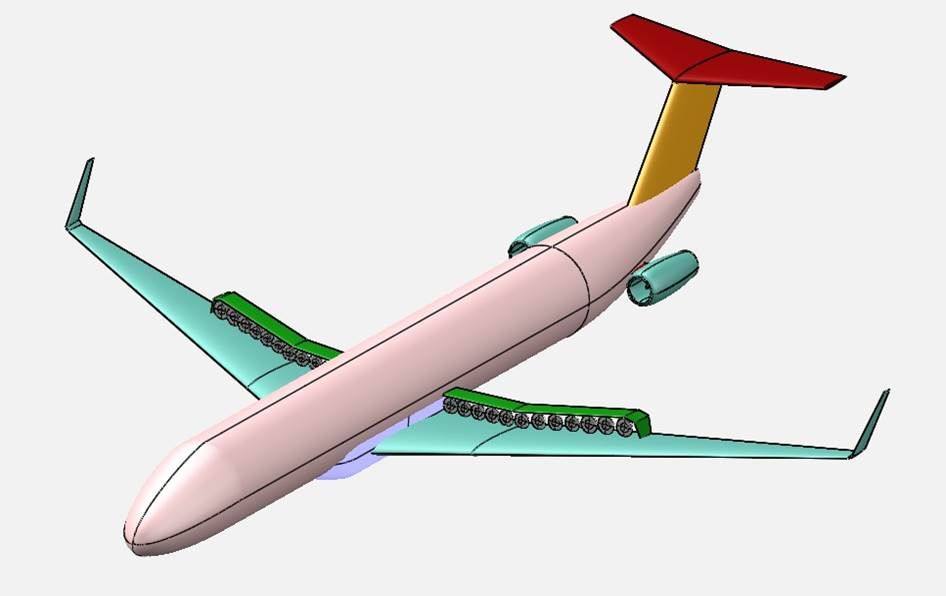
\includegraphics[width=0.5\textwidth]{aircraft_distributed_prop.png}\\
\vspace{-1cm}
{\hfill\tiny (from \cite{sgueglia2018exploration})}
\end{center}
\vskip\baselineskip
$x$ = aircraft parameters (here distributed electrical propulsion)\\
$f()$ = $-1\times$ performance metric (aggregation of $-1\times$ range, cost, take-off length, \ldots) \\
At the minimum, the design is ``optimal''.
\end{frame}


%%%%%%%%%%%%%%%%%%%%%%%%%%%%%%%%%%%%%%%%%%%%%%%%%%%%%%%%%%%%%%%%%
\begin{frame}
\frametitle{Optimization example: blade detailed design}
\begin{center}
\centering
\mbox{
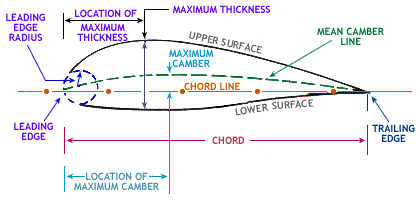
\includegraphics[width=0.33\linewidth]{Schema_Rotor}
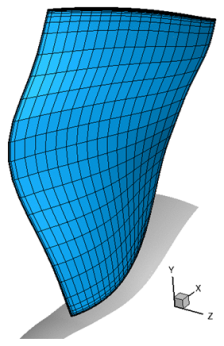
\includegraphics[width=0.13\linewidth]{blade}
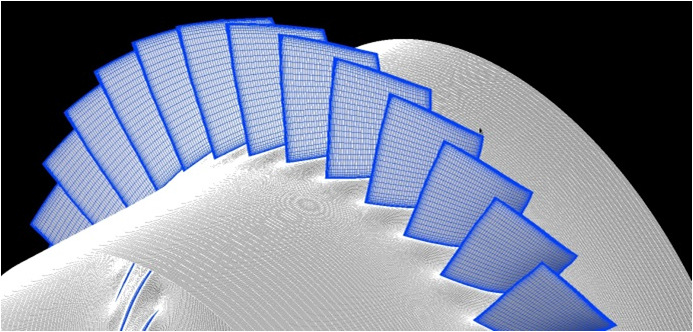
\includegraphics[width=0.33\linewidth]{rotor}
}
\end{center}
{\footnotesize
{\normalsize $x$:} The blades are described by 4 cross-sections for a total of 20 design parameters. 
\\
{\normalsize $f()$:} 5 constraints about the inlet and outlet relative flow angles, the flow speed reduction, excessive loading and the Mach number of the blade tips.
The objective function is the polytropic (compressor) efficiency. From \cite{roustant:hal-03217277}.
}
\vskip\baselineskip
Favorable application: non-intuitive design and a small gain makes a large difference.
\end{frame}

%%%%%%%%%%%%%%%%%%%%%%%%%%%%%%%%%%%%%%%%%%%%%%%%%%%%%%%%%%%%%%%%%
\begin{frame}
\frametitle{Optimization example: composite structure design}
\begin{center}
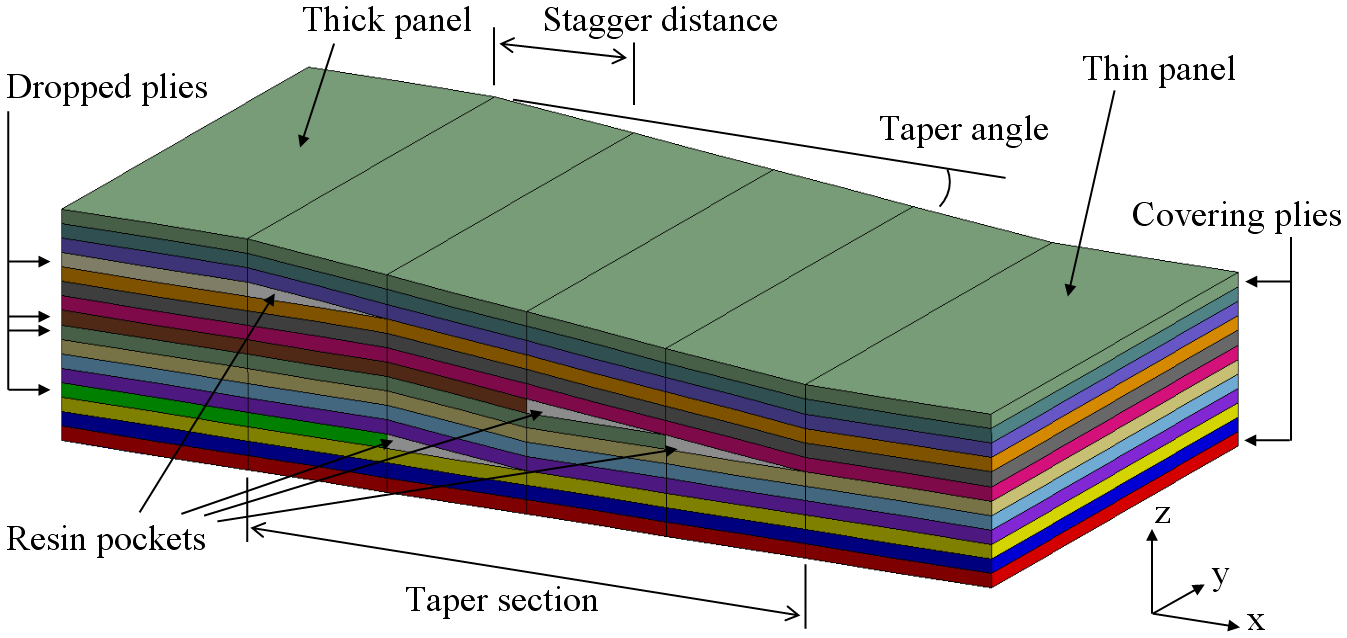
\includegraphics[width=0.7\textwidth]{ply_drop.png}
\end{center}
$x$ is the orientation of the fibers within the plies of a composite laminate and the location where the plies are dropped.
\\
$f()$ mechanical performance (stiffness, low mass, strength, stability, \ldots)
\\
Many arrangements of the $x$'s have almost equivalent performances, leading to local optima
(from \cite{irisarri2014optimal}).
\end{frame}

%%%%%%%%%%%%%%%%%%%%%%%%%%%%%%%%%%%%%%%%%%%%%%%%%%%%%%%%%%%%%%%%%
\begin{frame}
\frametitle{Optimization example: model identification}
\begin{center}
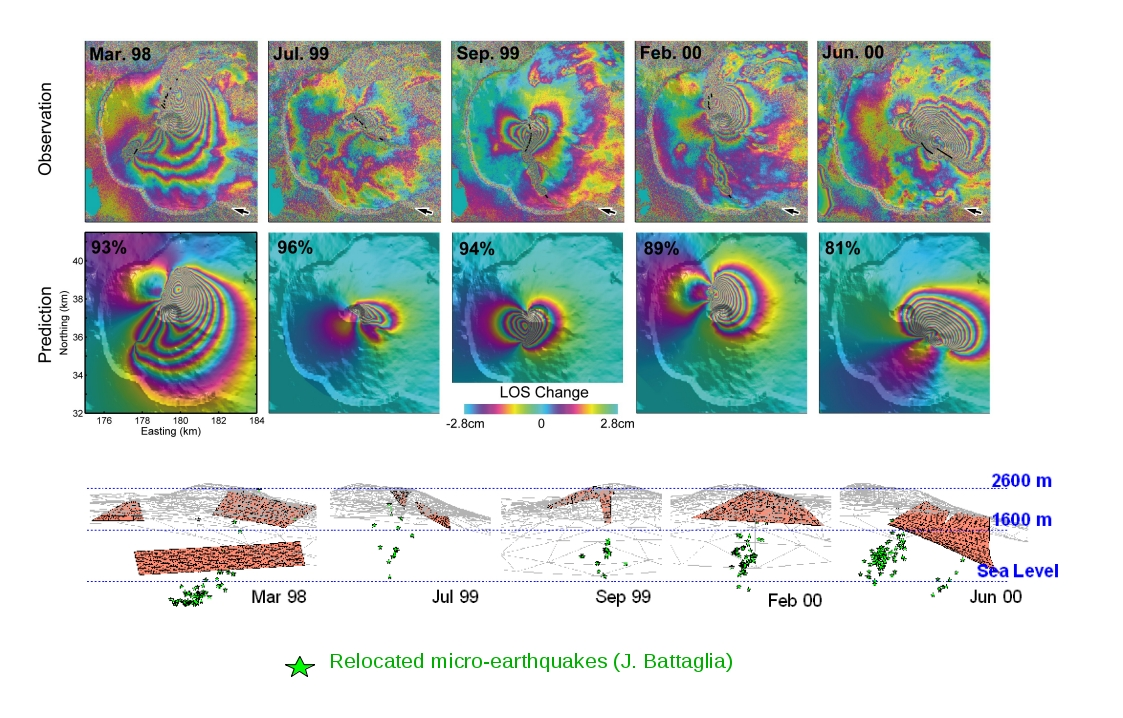
\includegraphics[width=0.7\textwidth]{piton_fournaise.jpg}\\
\vspace{-1cm}
{\hfill\tiny (from \cite{fukushima2010evolution})}
\end{center}
$x$ = dike position, geometry, internal pressure\\
$f()$ = distance between measures (from RADARSAT-1 satellite) and model (boundary elements, non trivial computation)\\
At the minimum, the model best matches measurements and should correspond to the underground phenomenon.
\end{frame}

%%%%%%%%%%%%%%%%%%%%%%%%%%%%%%%%%%%%%%%%%%%%%%%%%%%%%%%%%%%%%%%%%
\begin{frame}
\frametitle{Optimization example: wind farm layout}
\begin{center}
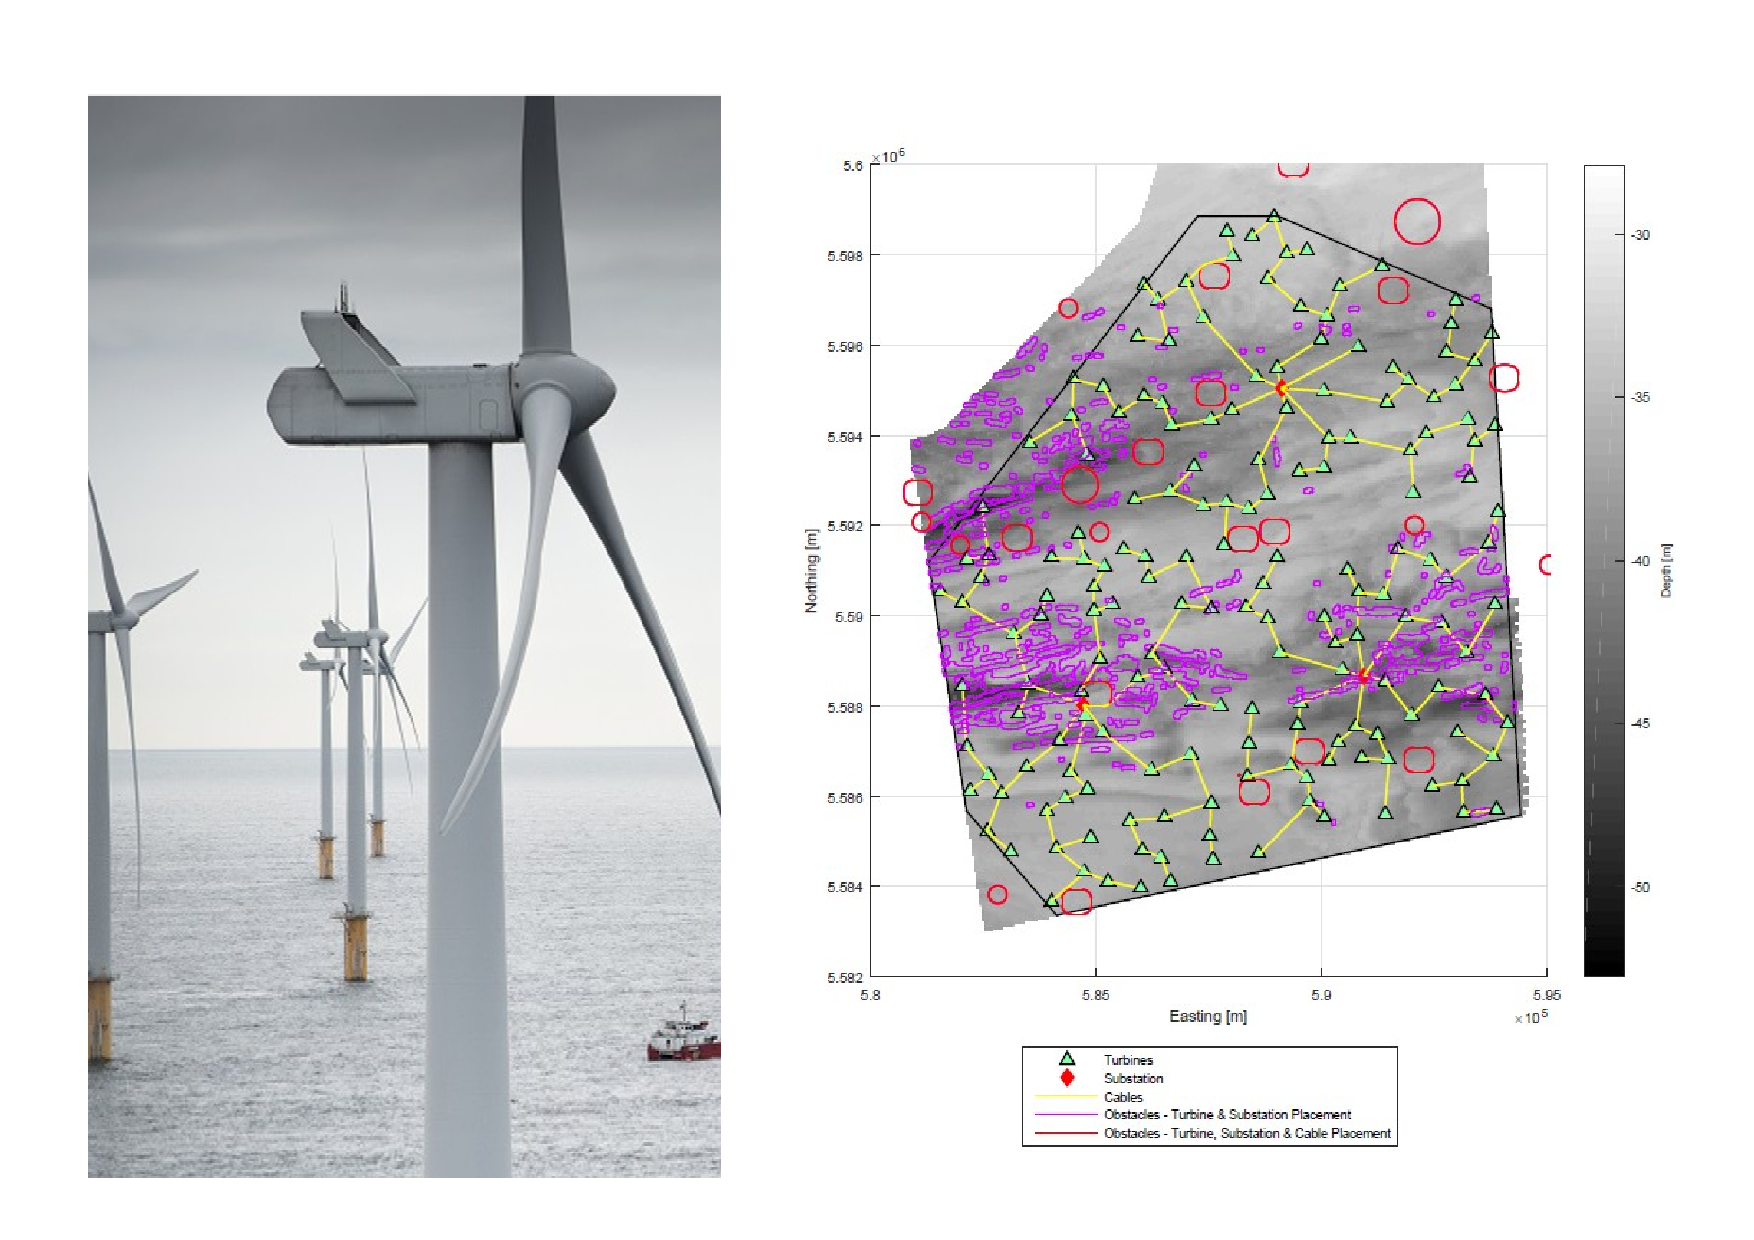
\includegraphics[width=0.7\textwidth]{wind_farm_model.pdf}
\end{center}
$x$ = position and characteristics of the wind mill, electrical network.
$f()$ = cost aggregated with -1 $\times$ average power production.
\end{frame}

%%%%%%%%%%%%%%%%%%%%%%%%%%%%%%%%%%%%%%%%%%%%%%%%%%%%%%%%%%%%%%%%%
\begin{frame}
\frametitle{Optimization example: image denoising}
\vspace{-0.5cm}
\begin{equation*}
\begin{split}
\min_x f(x) \quad,\quad & f(x) = \frac{1}{2}\sum_{i=1}^{N_{\text{pixels}}} (y_i - x_i)^2 + 
\lambda \sum_{i=1}^{N_{\text{pixels}}} \sum_{j \text{ near } i} \lvert x_i - x_j \rvert \\
& \lambda \ge 0 \quad\text{regularization constant}
\end{split}
\end{equation*}
\begin{center}
\begin{minipage}[t]{0.2\textwidth}

\includegraphics[width=\textwidth]{c_clean.png} \\
{\small target image}
\end{minipage}
\hfill
\begin{minipage}[t]{0.2\textwidth}

\includegraphics[width=\textwidth]{c_noisy.png} \\
{\small \mbox{noisy (observed)} $= y_i$'s}
\end{minipage}
\hfill
\begin{minipage}[t]{0.2\textwidth}

\includegraphics[width=\textwidth]{c_denoised.png} \\
{\small \mbox{denoised (optimized)} $=x^\star$}
\end{minipage}
\mbox{\quad}
\end{center}
{\scriptsize (from \cite{ravikumar17}) \hfill}
\end{frame}

%%%%%%%%%%%%%%%%%%%%%%%%%%%%%%%%%%%%%%%%%%%%%%%%%%%%%%%%%%%%%%%%%
\begin{frame}
\frametitle{Optimization example: neural net learning}
\begin{minipage}{0.5\textwidth}
$x$ = neural network (NN) weights and biases
\vskip\baselineskip
$f()$ = an error of the NN predictions w.r.t. data (a loss function)
\end{minipage}
\hfill
\begin{minipage}{0.4\textwidth}
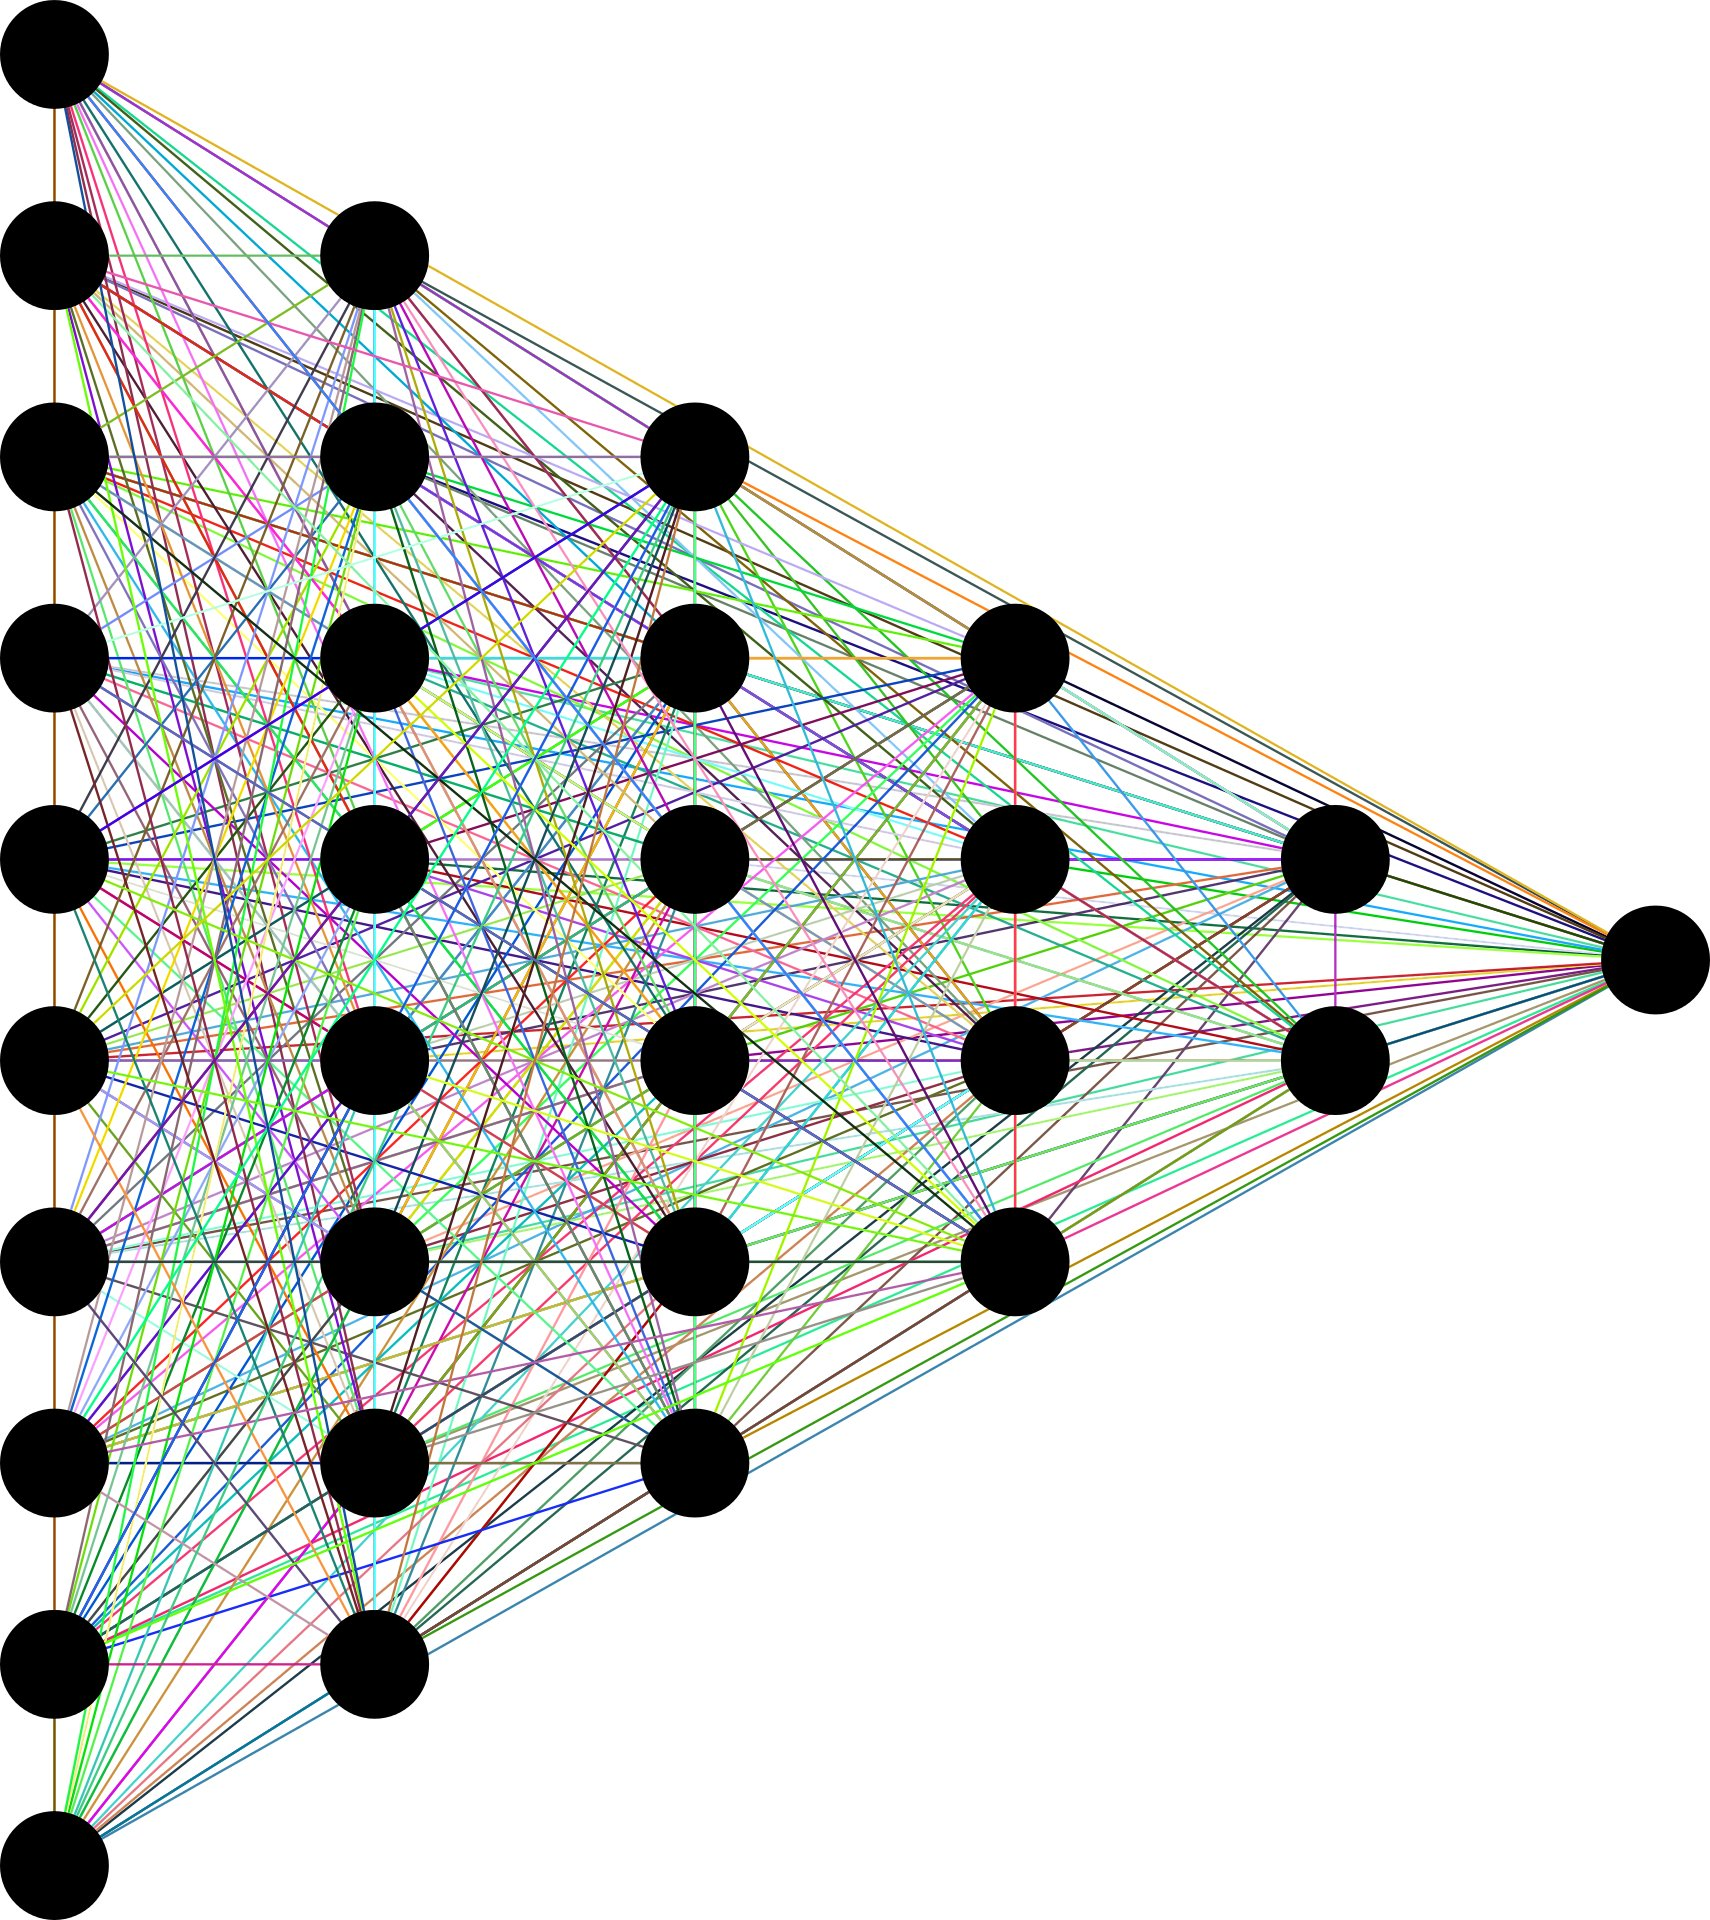
\includegraphics[width=\textwidth]{neuralnetwork_CC0_public_domain.jpg} \\
{\tiny from \url{techxplore.com/news/2020-11-neural-network.html}, CC0 public domain \par}
\end{minipage}
\end{frame}



%%%%%%%%%%%%%%%%%%%%%%%%%%%%%%%%%%%%%%%%%%%%%%%%%%%%%%%%%%%%%%%%%
\begin{frame}
\frametitle{An utopia ? (part 1)}
Optimization as a mathematical model for decision
\vskip\baselineskip
\mbox{
\begin{minipage}[c]{0.2\textwidth}

\includegraphics[width=\textwidth]{decision-clipart.jpg}
\end{minipage}
\begin{minipage}[c]{0.7\textwidth}
\begin{equation*}
\min_{x \in \mathcal S} f(x)
\end{equation*}
\end{minipage}
} % end mbox
\vskip\baselineskip
Don't forget the human in the loop ! 
\begin{itemize}
\item In \cite{tsoukias2008decision}, broader framework (model of the human rationality) $\Rightarrow$ decision \alert{aiding} theory.
\item Multi-Disciplinary Optimization \cite{brevault2020aerospace} as an attempt to model interacting disciplines.
\item Human systems are complex, not easy to model.
\end{itemize}
\begin{block}{}
Here, modest and practical goal : optimization as a (fascinating) \alert{tool}.
\end{block}
\end{frame}


%%%%%%%%%%%%%%%%%%%%%%%%%%%%%%%%%%%%%%%%%%%%%%%%%%%%%%%%%%%%%%%%%
\begin{frame}[allowframebreaks]
\frametitle{Historical and epistemological hints}
Emergence conditions : optimization algorithms have become a scientific subject of its own when the problem to solve has been decomposed into 
\begin{itemize}
\item a real object to optimize,
\item a space of representations $\mathcal S$ where $x$ is chosen,
\item a performance model $f(x)$,
\item a motion principle (the optimization algorithm).
\end{itemize}
\pagebreak
Optimization problems were solved before, but in a unified manner: 
\vskip\baselineskip
\mbox{
\begin{minipage}{0.4\textwidth}
The Brachistochrone curve: minimize time to go from A to B with a frictionless ball under the action of gravity.
Posed and solved by Johann Bernoulli in 1696.
\end{minipage}
\begin{minipage}{0.5\textwidth}
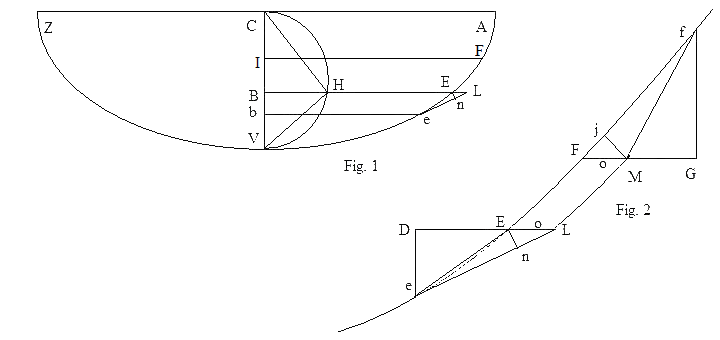
\includegraphics[width=\textwidth]{Bernoulli_Challenge_to_Newton_1.png} \\
\end{minipage}
}
\pagebreak
\begin{minipage}{0.4\textwidth}
Hooke's theorem (1675) :\\
``As hangs the flexible chain, so but inverted will stand the rigid arch.''
\\
\begin{center}
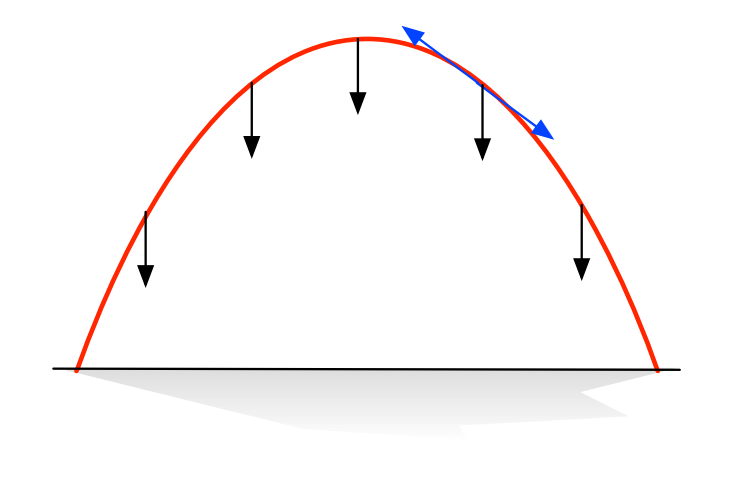
\includegraphics[width=0.45\textwidth]{arche.png}
\end{center}
\end{minipage}
\hfill
\begin{minipage}{0.4\textwidth}
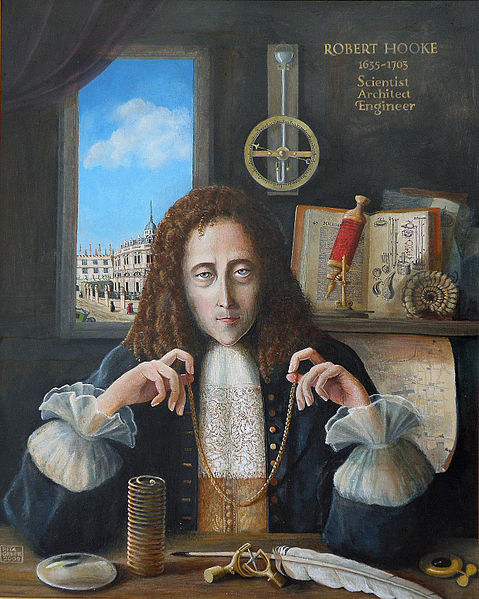
\includegraphics[width=\textwidth]{Robert-Hooke.jpeg} \\
{\tiny 
Robert Hooke holding a chain that forms a catenary curve. 
Image by Rita Greer. Licensed under Free Art License 1.3, via Wikimedia Commons.}
\end{minipage}


\begin{block}{A decomposition principle in science}
Elements of scientific knowledge appear in relation to a problem that is sufficiently decomposed.
\end{block}
Close to Descartes' 2nd Rule in Discourse on the Method : ``Divide each difficulty into as many parts as is feasible and necessary to resolve it''
(but more on a spontaneous architecture of a problem).\\

\end{frame}

\section{Bibliography}

%=======================================================================================
\begin{frame}[allowframebreaks]
\frametitle{References}
\scriptsize
%\vspace{-1.cm}
%\setbeamertemplate{bibliography item}{[\theenumiv]} % to have numbers in biblio with beamer
%   \bibliographystyle{plain}
   \bibliographystyle{apalike}
   \bibliography{biblio}
\end{frame}

\end{document}

